\section{\KIM}
\begin{frame}{Algoritmo de Katoh, Ibaraki e Mine}
	\begin{itemize}
		\item<1-> Espec�fico para grafos sim�tricos
		\item<2-> M�todo eficiente para o problema do desvio m�nimo
		\item<3-> Diminui��o do n�mero de caminhos candidatos gerados a cada itera��o
		\item<4-> Baseado no m�todo de Yen
		\item<5-> Parti��es definidas apenas para n�s com mais de um filho
		\item<6-> Depende rotina para o problema \PCM{}: $T(n,m)$
		\item<7-> Melhor desempenho assint�tico: $\Theta(kT(n,m))$
	\end{itemize}
\end{frame}

%% \begin{frame}{Teste}
%% \begin{tikzpicture}[style=thick]
%% \foreach \x in {0,1,2}
%% \foreach \y in {0,1,2}
%% {\draw (\y,0) -- (\x,1);}
%% \foreach \x in {0,1,2}{
%% \draw (\x,0) circle (2pt);
%% \draw (\x,1) circle (2pt);}
%% \end{tikzpicture}
%% 
%%         %\begin{figure}
%% 	%\pgfuseimage{kimCaminhos}
%% 	%\end{figure}
%% \end{frame}
%% 
%% 
%% \begin{frame}{Tabela}
%% 
%%   \begin{tikzpicture}[node distance=2cm]
%% \SetUpEdge[lw         = 1.5pt,
%% %              color      = black,
%% %              labelcolor = blue,
%% %              labeltext  = red,
%% %             labelstyle = {above,pos=.5,text=blue}
%%             ]
%%   \GraphInit[vstyle=Shade]
%%     \tikzset{LabelStyle/.style =   {                                   
%%                                   text  = red, font=\tiny}}
%%   \Vertex{a}
%%   \EA(a){b}
%%   \EA(b){d}
%%   \EA(d){e}
%%   \SOEA(b){c}
%%   \Edge[style={>=latex},label=1](a)(b)
%%   \Edge[label=1](b)(c)
%%   \Edge[label=1.0](b)(c)
%%   \Edge[label=1](c)(d)
%%   \Edge[label=1.0](d)(e)
%%   \Edge[label=0](b)(d)
%%   \end{tikzpicture}
%%   \begin{tikzpicture}[node distance=2cm]
%% \SetUpEdge[lw         = 1.5pt,
%% %              color      = black,
%% %              labelcolor = blue,
%% %              labeltext  = red,
%% %             labelstyle = {above,pos=.5,text=blue}
%%             ]
%%   \GraphInit[vstyle=Shade]
%%     \tikzset{LabelStyle/.style =   {                                   
%%                                   text  = red, font=\tiny}}
%%   \Vertex{a}
%%   \EA(a){b}
%%   \EA(b){d}
%%   \EA(d){e}
%%   \SOEA(b){c}
%%   \Edge[style={>=latex},label=1](a)(b)
%%   \Edge[label=1](b)(c)
%%   \Edge[label=1.0](b)(c)
%%   \Edge[label=1](c)(d)
%%   \Edge[label=1.0](d)(e)
%%   \Edge[label=0](b)(d)
%%   \end{tikzpicture}
%%   
%%     \begin{tikzpicture}[node distance=2cm]
%% 	\SetUpEdge[lw         = 1.5pt,
%% %              color      = black,
%% %              labelcolor = blue,
%% %              labeltext  = red,
%% %             labelstyle = {above,pos=.5,text=blue}
%%             ]
%%   \GraphInit[vstyle=Shade]
%%     \tikzset{LabelStyle/.style =   {                                   
%%                                   text  = red, font=\tiny}}
%%   \Vertex{a}
%%   \EA(a){b}
%%   \EA(b){d}
%%   \EA(d){e}
%%   \SOEA(b){c}
%%   \Edge[style={>=latex},label=1](a)(b)
%%   \Edge[label=1](b)(c)
%%   \Edge[label=1.0](b)(c)
%%   \Edge[label=1](c)(d)
%%   \Edge[label=1.0](d)(e)
%%   \Edge[label=0](b)(d)
%%   \end{tikzpicture}
%% 
%% \end{frame}
%% 
%% 
%% \begin{frame}
%% \frametitle{Prim's algorithm}
%% 
%% %% Adjacency matrix of graph
%% %% \  a  b  c  d  e  f  g
%% %% a  x  7     5
%% %% b  7  x  8  9  7
%% %% c     8  x     5
%% %% d  5  9     x 15  6
%% %% e     7  5 15  x  8  9
%% %% f           6  8  x 11
%% %% g              9  11 x
%% 
%% 
%% \tikzstyle{vertex}=[circle,fill=black!25,minimum size=20pt,inner sep=0pt]
%% \tikzstyle{selected vertex} = [vertex, fill=red!24]
%% \tikzstyle{edge} = [draw,thick,-]
%% \tikzstyle{weight} = [font=\small]
%% \tikzstyle{selected edge} = [draw,line width=5pt,-,red!50]
%% \tikzstyle{ignored edge} = [draw,line width=5pt,-,black!20]
%% 
%% 
%% \begin{figure}
%% \begin{tikzpicture}[scale=1.8, auto,swap]
%%     % Draw a 7,11 network
%%     % First we draw the vertices
%%     \foreach \pos/\name in {{(0,2)/a}, {(2,1)/b}, {(4,1)/c},
%%                             {(0,0)/d}, {(3,0)/e}, {(2,-1)/f}, {(4,-1)/g}}
%%         \node[vertex] (\name) at \pos {$\name$};
%%     % Connect vertices with edges and draw weights
%% 
%%  %   \foreach \source/ \dest /\weight in {b/a/7, c/b/8,d/a/5,d/b/9,
%%   %                                       e/b/7, e/c/5,e/d/15,
%%    %                                      f/d/6,f/e/8,
%%     %                                     g/e/9,g/f/11}
%% %        \path[edge] (\source) -- node[weight] {$\weight$} (\dest);
%%         
%%         \path[edge] (a) -- node[weight] {$7$} (b);
%%         \path[edge] (a) -- node[weight] {$5$} (d);
%%     % Start animating the vertex and edge selection. 
%% 
%% %    \foreach \vertex / \fr in {d/1,a/2,f/3,b/4,e/5,c/6,g/7}
%% %        \path<\fr-> node[selected vertex] at (\vertex) {$\vertex$};
%% 
%%     % For convenience we use a background layer to highlight edges
%%     % This way we don't have to worry about the highlighting covering
%%     % weight labels. 
%% 
%%  %   \begin{pgfonlayer}{background}
%%  %       \pause
%%  %       \foreach \source / \dest in {d/a,d/f,a/b,b/e,e/c,e/g}
%%  %           \path<+->[selected edge] (\source.center) -- (\dest.center);
%%  %       \foreach \source / \dest / \fr in {d/b/4,d/e/5,e/f/5,b/c/6,f/g/7}
%%  %           \path<\fr->[ignored edge] (\source.center) -- (\dest.center);
%%  %  \end{pgfonlayer}
%%     
%% \end{tikzpicture}
%% \end{figure}
%% 
%% \end{frame}

\begin{frame}{Exemplo �rvore dos menores caminhos}
\begin{columns}
\column{.6\textwidth}
\tikzstyle{vertex}=[circle,fill=black!25,minimum size=15pt,inner sep=0pt]
\tikzstyle{start} = [vertex, fill=red!24]
\tikzstyle{end} = [vertex, fill=red!24]
\tikzstyle{edge} = [draw,thick,-]
\tikzstyle{weight} = [font=\tiny]
\tikzstyle{selected edge} = [draw,line width=2pt,-,red!50]
\tikzstyle{not used} = [draw,line width=2pt,-,blue!50]
	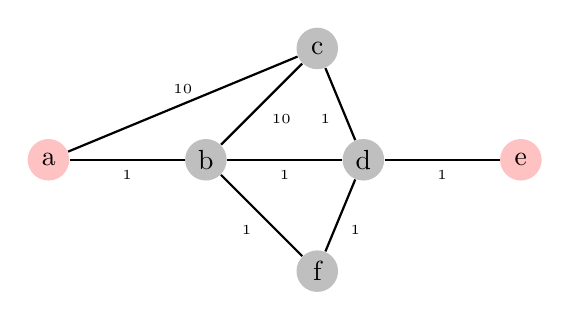
\begin{tikzpicture}[scale=1.0, auto,swap,node distance=2cm]
        \node[start] (a) {a};
        \node[vertex] (b) [right of=a] {b};
        \node[vertex] (c) [above right of=b] {c};
        \node[vertex] (d) [right of=b] {d};
        \node[vertex] (f) [below right of=b] {f};
        \node[end] (e) [right of=d] {e};
          
         \path[edge] (a) -- node[weight] {$1$} (b);
         \path[edge] (b) -- node[weight] {$1$} (d);
         \path[edge] (d) -- node[weight] {$1$} (e);
         \path[edge] (a) -- node[weight,above] {$10$} (c);
         \path[edge] (b) -- node[weight] {$10$} (c);
         \path[edge] (c) -- node[weight] {$1$} (d);
         \path[edge] (b) -- node[weight] {$1$} (f);
         \path[edge] (f) -- node[weight] {$1$} (d);
         
   \end{tikzpicture}

 
%%%%%%%%%%%%%%%%%%%%%%%%%%%%%%%%%%%%%%%%%%%%%%%%%%%%%%%%%%%%%%%%%%%%%%%%%%%%%
\column{.4\textwidth}
\tikzstyle{node}=[circle,fill=black!25,minimum size=10pt,inner sep=0pt]
\tikzstyle{root} = [node, fill=red!24]
\tikzstyle{leaf} = [node, fill=gray!24]
\tikzstyle{onPath} = [node, fill=red!24]
\tikzstyle{edge} = [draw,thick,-]
\tikzstyle{weight} = [font=\tiny]
\tikzstyle{selected edge} = [draw,thick,-,red!50]
%\tikzstyle{LabelStyle}=[fill=white,sloped]
\onslide<2->{
\begin{tikzpicture}[scale=0.9]
% Set the overall layout of the tree
\tikzstyle{level 1}=[level distance=1.5cm, sibling distance=2.5cm]
\tikzstyle{level 2}=[level distance=1.5cm, sibling distance=2.5cm]
  	\node[root] (a) {a} [grow=down,-] 
  	    child {
				node[node] (ab) {b}
				child[grow=south west]{
						node[node] (abd){d} 
						child[grow=south west]{
							node[node] (abde) {e}
							edge from parent
							node[left,weight] {1}
						}
						child[grow=south east] {
							node[node] {c}
							edge from parent
							node[right,weight] {1}
	 					}
						edge from parent
						node[left,weight] {1}
				}
				child[grow=south east]{
					node[node] {f} 
					edge from parent
					node[left,weight] {1}
				}				
				edge from parent
				node[left,weight] {1}
	 };
	\end{tikzpicture}
\tikzstyle{node}=[circle,fill=black!25,minimum size=10pt,inner sep=0pt]
\tikzstyle{root} = [node, fill=red!24]
\tikzstyle{leaf} = [node, fill=red!24]
\tikzstyle{onPath} = [node, fill=red!24]
\tikzstyle{edge} = [draw,thick,-]
\tikzstyle{weight} = [font=\tiny]
\tikzstyle{selected edge} = [draw,thick,-,red!50]
}
\onslide<3->{
%\tikzstyle{LabelStyle}=[fill=white,sloped]
\begin{tikzpicture}[scale=0.9]
% Set the overall layout of the tree
\tikzstyle{level 1}=[level distance=1.5cm, sibling distance=2.5cm]
\tikzstyle{level 2}=[level distance=1.5cm, sibling distance=2.5cm]
  	\node[root] (e) {e} [grow=up,-] 
  	    child {
				node[node]  (ed) {d} 
				child[grow=north west]{
						node[node] (edb) {b}  
						child{
							node[node] (edba) {a} 
							edge from parent
							node[left,weight] {1}
						}
						edge from parent
						node[left,weight] {1}
				}
				child {
							node[node] {c}
							edge from parent
							node[left,weight] {1}
	 					}
				child[grow=north east] {
							node[node] {f}
							edge from parent
							node[left,weight] {1}
	 					}
				edge from parent
				node[left,weight] {1}
	 }
	     ;
	\end{tikzpicture}
}

\end{columns}
\end{frame}


\subsection*{Problema do desvio de custo m�nimo}
\begin{frame}{Defini��o}
  \begin{quote}
    \textbf{Problema do desvio de custo m�nimo} $(V,A,c,s,t)$:\\
   Dados: 	
 	\begin{itemize}   
 	\item \small Grafo sim�trico com custo: $(V,A,c)$
 	\item V�rtices: $s$ e $t$ 
 	\item $P=\seq{s=a_1,\ldots,a_{n}=t}$ um caminho de custo m�nimo de $s$ a $t$
% 	\item $P_r=\seq{t = a_n , \ldots , a_{1} = s }$
% 	\item $T_s$ uma �rvore de menores caminhos com raiz em $s$
% 	\item $T_t$ uma �rvore de menores caminhos com raiz em $t$
% 	\item $P \in T_s$ e $P_r \in T_t$
	\end{itemize}	
	Encontrar um caminho de custo m�nimo, diferente de $P$, entre $s$ e $t$.
	\end{quote}
\end{frame}


\begin{frame}{Exemplo}

\tikzstyle{vertex}=[circle,fill=black!25,minimum size=15pt,inner sep=0pt]
\tikzstyle{start} = [vertex, fill=red!24]
\tikzstyle{end} = [vertex, fill=red!24]
\tikzstyle{edge} = [draw,thick,-]
\tikzstyle{weight} = [font=\tiny]
\tikzstyle{selected edge} = [draw,line width=2pt,-,red!50]
\tikzstyle{not used} = [draw,line width=2pt,-,blue!50]
\only<1>{
	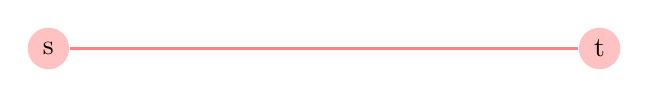
\begin{tikzpicture}[scale=1.0, auto,swap,node distance=7cm]
        \node[start] (s) {s};
        \node[end] (t) [right of=s] {t};
        
         \path[selected edge] (s) -- node[weight] {} (t);
        
   \end{tikzpicture}
}
\onslide<2->{
	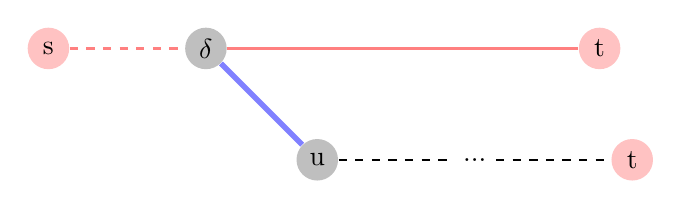
\begin{tikzpicture}[scale=1.0, auto,swap,node distance=2cm]
        \node[start] (s) {s};
        \node[vertex] (desvio) [right of=s] {$\delta$};
        \node[vertex] (u) [below right of=desvio] {u};
        \node (aux) [right of=u] {...};       
        \node[end,node distance=5cm] (t) [right of=desvio] {t};
        \node[end] (t2) [right of=aux] {t};
          
         \path[selected edge,dashed] (s) -- node[weight] {} (desvio);
         \path[selected edge] (desvio) -- node[weight] {} (t);
         \path[not used] (desvio) -- node[weight] {} (u);
         \path[edge,dashed] (u) -- node[weight,dashed] {} (aux);
         \path[edge,dashed] (aux) -- node[weight,dashed] {} (t2);
         
   \end{tikzpicture}
}
\onslide<3->{
	\begin{itemize}
	\item<3-> arco $\delta u \in T_s$
		\begin{itemize}
		\item<4-> $s \underset{T_s}{\longrightarrow} u \underset{T_t}{\longrightarrow} t$
		\end{itemize}
	\item<3-> arco $\delta u \notin T_s$
		\begin{itemize}
			\item<5-> $s \underset{T_s}{\longrightarrow} u \underset{\in A}{\rightarrow} v \underset{T_t}{\longrightarrow} t$
		\end{itemize}

	\end{itemize}
}
\end{frame}

\begin{frame}{Tipos de caminhos}
Um novo caminho de custo m�nimo constru�do atrav�s de $u \in V$ � de um dos dois tipos definidos a seguir:
\begin{description}
\item[tipo I]: $s \underset{T_s}{\longrightarrow} u \underset{T_t}{\longrightarrow} t$.  %Se $\epsilon(u)<\zeta(u)$
\newline
\item[tipo II]: $s \underset{T_s}{\longrightarrow} u \underset{\in A}{\rightarrow} v \underset{T_t}{\longrightarrow} t$. %Se $\epsilon(u)=\zeta(u)$ e $\epsilon(u)<\zeta(v)$
\end{description}

\begin{itemize}
\item $T_s$ uma �rvore de menores caminhos com raiz em $s$
\item $T_t$ uma �rvore de menores caminhos com raiz em $t$
\item $P_r=\seq{t = a_n , \ldots , a_{1} = s }$
\item $P \in T_s$ e $P_r \in T_t$
\end{itemize}
\end{frame}

\begin{frame}{Desvio de custo m�nimo}
%%%%%%%%%%%%%%%%%%%%%%%%%%%%%%%%%%%%%%%%%%%%%%%%%%%%%%%%%%%%%%%%%%%%%%%%%%%%%%%%%%%
%%%%%%%%%%%%%%%%%%%%%%%%%%%%%%%%%%grafo%%%%%%%%%%%%%%%%%%%%%%%%%%%%%%%%%%%%%%%%%%%5
%%%%%%%%%%%%%%%%%%%%%%%%%%%%%%%%%%%%%%%%%%%%%%%%%%%%%%%%%%%%%%%%%%%%%%%%%%%%%%%%%%%
\begin{columns}
\column{.6\textwidth}
\tikzstyle{vertex}=[circle,fill=black!25,minimum size=15pt,inner sep=0pt]
\tikzstyle{start} = [vertex, fill=red!24]
\tikzstyle{end} = [vertex, fill=red!24]
\tikzstyle{edge} = [draw,thick,-]
\tikzstyle{weight} = [font=\tiny]
\tikzstyle{selected edge} = [draw,line width=2pt,-,red!50]
\tikzstyle{not used} = [draw,line width=2pt,-,blue!50]
\only<1>{
	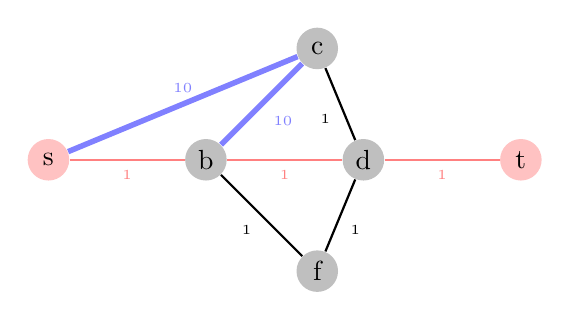
\begin{tikzpicture}[remember picture=false,scale=1.0, auto,swap,node distance=2cm]
        \node[start] (s) {s};
        \node[vertex] (b) [right of=s] {b};
        \node[vertex] (c) [above right of=b] {c};
        \node[vertex] (d) [right of=b] {d};
        \node[vertex] (f) [below right of=b] {f};
        \node[end] (t) [right of=d] {t};
          
         \path[selected edge] (s) -- node[weight] {$1$} (b);
         \path[selected edge] (b) -- node[weight] {$1$} (d);
         \path[selected edge] (d) -- node[weight] {$1$} (t);
         \path[not used] (s) -- node[weight,above] {$10$} (c);
         \path[not used] (b) -- node[weight] {$10$} (c);
         \path[edge] (c) -- node[weight] {$1$} (d);
         \path[edge] (b) -- node[weight] {$1$} (f);
         \path[edge] (f) -- node[weight] {$1$} (d);
         
   \end{tikzpicture}
}
\only<2>{
	\tikzstyle{novo} = [draw,line width=2pt,-,green!50]
	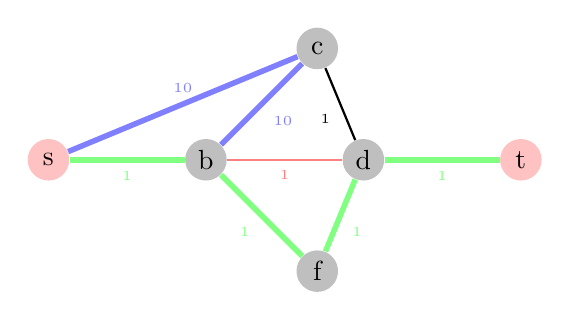
\begin{tikzpicture}[remember picture=false,scale=1.0, auto,swap,node distance=2cm]
        \node[start] (s) {s};
        \node[vertex] (b) [right of=s] {b};
        \node[vertex] (c) [above right of=b] {c};
        \node[vertex] (d) [right of=b] {d};
        \node[vertex] (f) [below right of=b] {f};
        \node[end] (t) [right of=d] {t};
          
         \path[novo] (s) -- node[weight] {$1$} (b);
         \path[novo] (b) -- node[weight] {$1$} (f);
         \path[novo] (f) -- node[weight] {$1$} (d);
         \path[novo] (d) -- node[weight] {$1$} (t);
         \path[selected edge] (b) -- node[weight] {$1$} (d);
         \path[not used] (s) -- node[weight,above] {$10$} (c);
         \path[not used] (b) -- node[weight] {$10$} (c);
         \path[edge] (c) -- node[weight] {$1$} (d);
   \end{tikzpicture}
}
\only<3>{
	\tikzstyle{novo} = [draw,line width=2pt,-,green!50]
	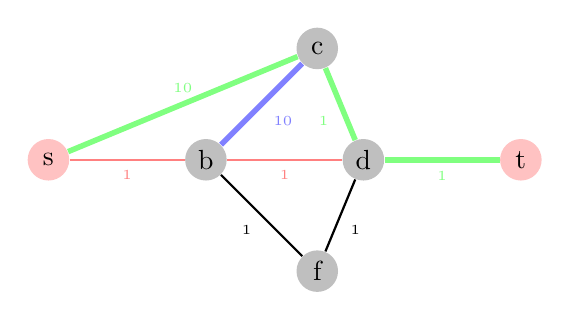
\begin{tikzpicture}[remember picture=false,scale=1.0, auto,swap,node distance=2cm]
        \node[start] (s) {s};
        \node[vertex] (b) [right of=s] {b};
        \node[vertex] (c) [above right of=b] {c};
        \node[vertex] (d) [right of=b] {d};
        \node[vertex] (f) [below right of=b] {f};
        \node[end] (t) [right of=d] {t};
          
         \path[selected edge] (s) -- node[weight] {$1$} (b);
         \path[selected edge] (b) -- node[weight] {$1$} (d);
         \path[novo] (d) -- node[weight] {$1$} (t);
         \path[novo] (s) -- node[weight,above] {$10$} (c);
         \path[not used] (b) -- node[weight] {$10$} (c);
         \path[novo] (c) -- node[weight] {$1$} (d);
         \path[edge] (b) -- node[weight] {$1$} (f);
         \path[edge] (f) -- node[weight] {$1$} (d);
   \end{tikzpicture}
}
\only<4>{
	\tikzstyle{novo} = [draw,line width=2pt,-,green!50]
	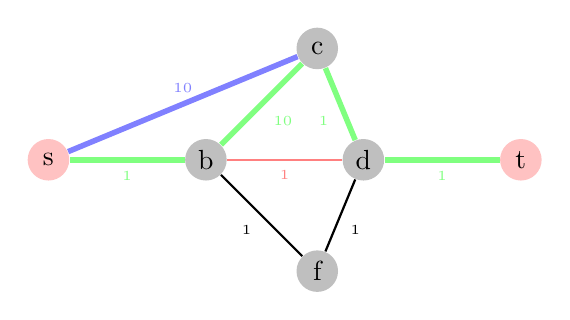
\begin{tikzpicture}[remember picture=false,scale=1.0, auto,swap,node distance=2cm]
        \node[start] (s) {s};
        \node[vertex] (b) [right of=s] {b};
        \node[vertex] (c) [above right of=b] {c};
        \node[vertex] (d) [right of=b] {d};
        \node[vertex] (f) [below right of=b] {f};
        \node[end] (t) [right of=d] {t};
          
         \path[novo] (s) -- node[weight] {$1$} (b);
         \path[selected edge] (b) -- node[weight] {$1$} (d);
         \path[novo] (d) -- node[weight] {$1$} (t);
         \path[not used] (s) -- node[weight,above] {$10$} (c);
         \path[novo] (b) -- node[weight] {$10$} (c);
         \path[novo] (c) -- node[weight] {$1$} (d);
         \path[edge] (b) -- node[weight] {$1$} (f);
         \path[edge] (f) -- node[weight] {$1$} (d);
   \end{tikzpicture}
}

   \begin{columns}[t]
   \column{.5\textwidth}
	
	\begin{block}{Tipo I}
	\begin{itemize}   
		\only<2>{\item \small \textcolor{green}{$\seq{s,b,f,d,t}$}}
		\onslide<3->{ \item \small $\seq{s,b,f,d,t}$ }
   \end{itemize}
	\end{block}   

   \column{.5\textwidth}

  	\begin{block}{Tipo II}
	\begin{itemize}   
		\only<3>{\item \small \textcolor{green}{$\seq{s,c,d,t}$}}
		\onslide<4->{\item \small $\seq{s,c,d,t}$}
		\onslide<4->{ \item \small \textcolor{green}{$\seq{s,b,c,d,t}$} }
   \end{itemize}
	\end{block} 
   \end{columns}
%	\begin{itemize}
%  	\only<3>{\item \small \textcolor{green}{$\seq{a,c,d,e}$}}
%  	\only<4>{\item \small \textcolor{green}{$\seq{a,b,c,d,e}$}}
%   \end{itemize}
   
%%%%%%%%%%%%%%%%%%%%%%%%%%%%%%%%%%%%%%%%%%%%%%%%%%%%%%%%%%%%%%%%%%%%%%%%%%%%%
\column{.4\textwidth}
\tikzstyle{node}=[circle,fill=black!25,minimum size=10pt,inner sep=0pt]
\tikzstyle{root} = [node, fill=red!24]
\tikzstyle{leaf} = [node, fill=red!24]
\tikzstyle{onPath} = [node, fill=red!24]
\tikzstyle{edge} = [draw,thick,-]
\tikzstyle{weight} = [font=\tiny]
\tikzstyle{selected edge} = [draw,thick,-,red!50]
%\tikzstyle{LabelStyle}=[fill=white,sloped]
\begin{tikzpicture}[remember picture=true,scale=0.9]
% Set the overall layout of the tree
\tikzstyle{level 1}=[level distance=1.5cm, sibling distance=2.5cm]
\tikzstyle{level 2}=[level distance=1.5cm, sibling distance=2.5cm]
  	\node[root] (a) {s} [grow=down,-] 
  	    child {
				node[onPath] (ab) {b}
				child[grow=south west]{
						node[onPath](abd){d} 
						child[grow=south west]{
							node[onPath] (abde) {t}
							edge from parent
							node[left,weight] {1}
						}
						child[grow=south east] {
							node[node] {c}
							edge from parent
							node[right,weight] {1}
	 					}
						edge from parent
						node[left,weight] {1}
				}
				child[grow=south east]{
					node[node] (abf) {f} 
					edge from parent
					node[left,weight] {1}
				}				
				edge from parent
				node[left,weight] {1}
	 };
  	\path[selected edge] (a) -- node[weight] {} (ab);
   \path[selected edge] (ab) -- node[weight] {} (abd);
   \path[selected edge] (abd) -- node[weight] {} (abde);   
	\end{tikzpicture}
\tikzstyle{node}=[circle,fill=black!25,minimum size=10pt,inner sep=0pt]
\tikzstyle{root} = [node, fill=red!24]
\tikzstyle{leaf} = [node, fill=red!24]
\tikzstyle{onPath} = [node, fill=red!24]
\tikzstyle{edge} = [draw,thick,-]
\tikzstyle{weight} = [font=\tiny]
\tikzstyle{selected edge} = [draw,thick,-,red!50]
%\tikzstyle{LabelStyle}=[fill=white,sloped]
\begin{tikzpicture}[remember picture=true,scale=0.9]
% Set the overall layout of the tree
\tikzstyle{level 1}=[level distance=1.5cm, sibling distance=2.5cm]
\tikzstyle{level 2}=[level distance=1.5cm, sibling distance=2.5cm]
  	\node[root] (e) {t} [grow=up,-] 
  	    child {
				node[onPath]  (ed) {d} 
				child[grow=north west]{
						node[onPath] (edb) {b}  
						child{
							node[onPath] (edba) {s} 
							edge from parent
							node[left,weight] {1}
						}
						edge from parent
						node[left,weight] {1}
				}
				child {
							node[node] (tdc) {c}
							edge from parent
							node[left,weight] {1}
	 					}
				child[grow=north east] {
							node[node] (tdf) {f}
							edge from parent
							node[left,weight] {1}
	 					}
				edge from parent
				node[left,weight] {1}
	 }
	     ;
 	\path[selected edge] (e) -- node[weight] {} (ed);
   \path[selected edge] (ed) -- node[weight] {} (edb);
   \path[selected edge] (edb) -- node[weight] {} (edba);
	\end{tikzpicture}
	\only<2>{
	\begin{tikzpicture}[remember picture=true,overlay,>=latex]
	 	\path[dashed,green] (abf) edge (tdf);
	\end{tikzpicture}
	}
	\only<3>{
	\begin{tikzpicture}[remember picture=true,overlay,>=latex]
	 	\path[dashed,green,bend left] (a) edge (tdc);
	\end{tikzpicture}
	}
		\only<4>{
	\begin{tikzpicture}[remember picture=true,overlay,>=latex]
	 	\path[dashed,green,bend left] (ab) edge (tdc);
	\end{tikzpicture}
	}

\end{columns}
\end{frame}


\begin{frame}{Rotula��es $\epsilon$ e $\zeta$}
\begin{center}
\textcolor{red}{$P=\seq{a,b,d,e}$}
\end{center}
\begin{columns}[c]
\column{.5\textwidth}
\begin{block}{Rotula��o $\epsilon$}
\small
$\epsilon(a)=1$ \\
Se $u \in P$ ent�o $\epsilon(u)=\epsilon(\pred(u))+1$ \\
Se $u \notin P$ ent�o $\epsilon(u)=\epsilon(\pred(u))$
\end{block}
\tikzstyle{node}=[circle,fill=black!25,minimum size=10pt,inner sep=0pt]
\tikzstyle{root} = [node, fill=red!24]
\tikzstyle{leaf} = [node, fill=red!24]
\tikzstyle{onPath} = [node, fill=red!24]
\tikzstyle{edge} = [draw,thick,-]
\tikzstyle{weight} = [font=\tiny]
\tikzstyle{selected edge} = [draw,thick,-,red!50]
%\tikzstyle{LabelStyle}=[fill=white,sloped]
\begin{tikzpicture}[scale=1.0]
% Set the overall layout of the tree
\tikzstyle{level 1}=[level distance=1.5cm, sibling distance=2.5cm]
\tikzstyle{level 2}=[level distance=1.5cm, sibling distance=2.5cm]
  	\node[root,label=right:{\footnotesize $\epsilon=1$}] (a) {a} [grow=down,-] 
  	    child {
				node[onPath,label=right:{\footnotesize $2$}] (ab) {b}
				child[grow=south west]{
						node[onPath,label=right:{\footnotesize $3$}](abd){d} 
						child[grow=south west]{
							node[onPath,label=left:{\footnotesize $4$}] (abde) {e}
							edge from parent
							node[left,weight] {}
						}
						child[grow=south east] {
							node[node,label=right:{\footnotesize $3$}] {c}
							edge from parent
							node[right,weight] {}
	 					}
						edge from parent
						node[left,weight] {}
				}
				child[grow=south east]{
					node[node,label=right:{\footnotesize $2$}] {f} 
					edge from parent
					node[left,weight] {}
				}				
				edge from parent
				node[left,weight] {}
	 };
  	\path[selected edge] (a) -- node[weight] {} (ab);
   \path[selected edge] (ab) -- node[weight] {} (abd);
   \path[selected edge] (abd) -- node[weight] {} (abde);   
	\end{tikzpicture}
\column{.5\textwidth}
\begin{block}{Rotula��o $\zeta$}
\small
$\zeta(e)=|P|$ \\
Se $u \in P$ ent�o $\zeta(u)=\zeta(\pred(u))-1$ \\
Se $u \notin P$ ent�o $\zeta(u)=\zeta(\pred(u))$
\end{block}
\tikzstyle{node}=[circle,fill=black!25,minimum size=10pt,inner sep=0pt]
\tikzstyle{root} = [node, fill=red!24]
\tikzstyle{leaf} = [node, fill=red!24]
\tikzstyle{onPath} = [node, fill=red!24]
\tikzstyle{edge} = [draw,thick,-]
\tikzstyle{weight} = [font=\tiny]
\tikzstyle{selected edge} = [draw,thick,-,red!50]
%\tikzstyle{LabelStyle}=[fill=white,sloped]
\begin{tikzpicture}[scale=1.0]
% Set the overall layout of the tree
\tikzstyle{level 1}=[level distance=1.5cm, sibling distance=2.5cm]
\tikzstyle{level 2}=[level distance=1.5cm, sibling distance=2.5cm]
  	\node[root,label=right:{\footnotesize $\zeta=4$}] (e) {e} [grow=up,-] 
  	    child {
				node[onPath,label=right:{\footnotesize $3$}]  (ed) {d} 
				child[grow=north west]{
						node[onPath,label=left:{\footnotesize $2$}] (edb) {b}  
						child{
							node[onPath,label=left:{\footnotesize $1$}] (edba) {a} 
							edge from parent
							node[left,weight] {}
						}
						edge from parent
						node[left,weight] {}
				}
				child {
							node[node,label=right:{\footnotesize $3$}] {c}
							edge from parent
							node[left,weight] {}
	 					}
				child[grow=north east] {
							node[node,label=right:{\footnotesize $3$}] {f}
							edge from parent
							node[left,weight] {}
	 					}
				edge from parent
				node[left,weight] {}
	 }
	     ;
 	\path[selected edge] (e) -- node[weight] {} (ed);
   \path[selected edge] (ed) -- node[weight] {} (edb);
   \path[selected edge] (edb) -- node[weight] {} (edba);
	\end{tikzpicture}
\end{columns}
\end{frame}


\begin{frame}{Desvio de custo m�nimo com rotula��es}
%%%%%%%%%%%%%%%%%%%%%%%%%%%%%%%%%%%%%%%%%%%%%%%%%%%%%%%%%%%%%%%%%%%%%%%%%%%%%%%%%%%
%%%%%%%%%%%%%%%%%%%%%%%%%%%%%%%%%%grafo%%%%%%%%%%%%%%%%%%%%%%%%%%%%%%%%%%%%%%%%%%%5
%%%%%%%%%%%%%%%%%%%%%%%%%%%%%%%%%%%%%%%%%%%%%%%%%%%%%%%%%%%%%%%%%%%%%%%%%%%%%%%%%%%
\begin{columns}
\column{.6\textwidth}
\tikzstyle{vertex}=[circle,fill=black!25,minimum size=15pt,inner sep=0pt]
\tikzstyle{start} = [vertex, fill=red!24]
\tikzstyle{end} = [vertex, fill=red!24]
\tikzstyle{edge} = [draw,thick,-]
\tikzstyle{weight} = [font=\tiny]
\tikzstyle{selected edge} = [draw,line width=2pt,-,red!50]
\tikzstyle{not used} = [draw,line width=2pt,-,blue!50]
\only<1>{
	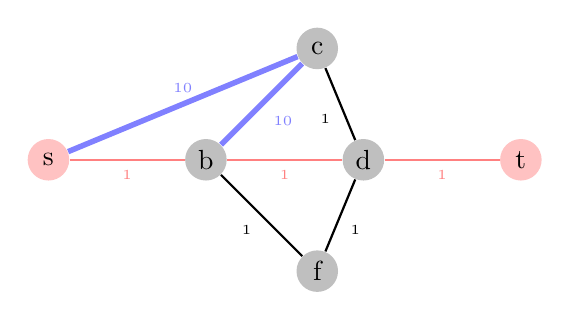
\begin{tikzpicture}[scale=1.0, auto,swap,node distance=2cm]
        \node[start] (a) {s};
        \node[vertex] (b) [right of=a] {b};
        \node[vertex] (c) [above right of=b] {c};
        \node[vertex] (d) [right of=b] {d};
        \node[vertex] (f) [below right of=b] {f};
        \node[end] (e) [right of=d] {t};
          
         \path[selected edge] (a) -- node[weight] {$1$} (b);
         \path[selected edge] (b) -- node[weight] {$1$} (d);
         \path[selected edge] (d) -- node[weight] {$1$} (e);
         \path[not used] (a) -- node[weight,above] {$10$} (c);
         \path[not used] (b) -- node[weight] {$10$} (c);
         \path[edge] (c) -- node[weight] {$1$} (d);
         \path[edge] (b) -- node[weight] {$1$} (f);
         \path[edge] (f) -- node[weight] {$1$} (d);
         
   \end{tikzpicture}
}
\only<2>{
	\tikzstyle{novo} = [draw,line width=2pt,-,green!50]
	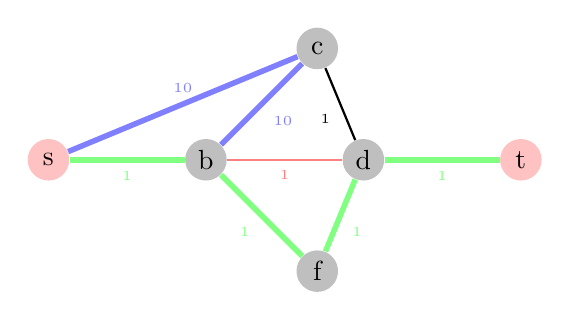
\begin{tikzpicture}[scale=1.0, auto,swap,node distance=2cm]
        \node[start] (a) {s};
        \node[vertex] (b) [right of=a] {b};
        \node[vertex] (c) [above right of=b] {c};
        \node[vertex] (d) [right of=b] {d};
        \node[vertex] (f) [below right of=b] {f};
        \node[end] (e) [right of=d] {t};
          
         \path[novo] (a) -- node[weight] {$1$} (b);
         \path[novo] (b) -- node[weight] {$1$} (f);
         \path[novo] (f) -- node[weight] {$1$} (d);
         \path[novo] (d) -- node[weight] {$1$} (e);
         \path[selected edge] (b) -- node[weight] {$1$} (d);
         \path[not used] (a) -- node[weight,above] {$10$} (c);
         \path[not used] (b) -- node[weight] {$10$} (c);
         \path[edge] (c) -- node[weight] {$1$} (d);
   \end{tikzpicture}
}
\only<3>{
	\tikzstyle{novo} = [draw,line width=2pt,-,green!50]
	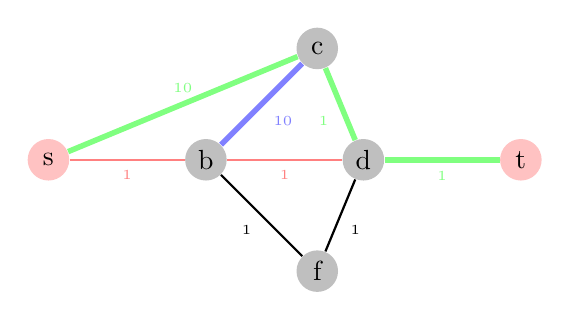
\begin{tikzpicture}[scale=1.0, auto,swap,node distance=2cm]
        \node[start] (a) {s};
        \node[vertex] (b) [right of=a] {b};
        \node[vertex] (c) [above right of=b] {c};
        \node[vertex] (d) [right of=b] {d};
        \node[vertex] (f) [below right of=b] {f};
        \node[end] (e) [right of=d] {t};
          
         \path[selected edge] (a) -- node[weight] {$1$} (b);
         \path[selected edge] (b) -- node[weight] {$1$} (d);
         \path[novo] (d) -- node[weight] {$1$} (e);
         \path[novo] (a) -- node[weight,above] {$10$} (c);
         \path[not used] (b) -- node[weight] {$10$} (c);
         \path[novo] (c) -- node[weight] {$1$} (d);
         \path[edge] (b) -- node[weight] {$1$} (f);
         \path[edge] (f) -- node[weight] {$1$} (d);
   \end{tikzpicture}
}
\only<4>{
	\tikzstyle{novo} = [draw,line width=2pt,-,green!50]
	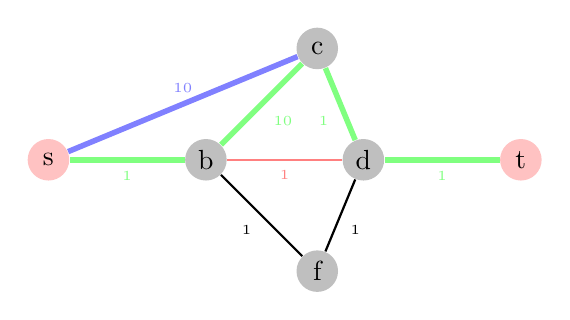
\begin{tikzpicture}[scale=1.0, auto,swap,node distance=2cm]
        \node[start] (a) {s};
        \node[vertex] (b) [right of=a] {b};
        \node[vertex] (c) [above right of=b] {c};
        \node[vertex] (d) [right of=b] {d};
        \node[vertex] (f) [below right of=b] {f};
        \node[end] (e) [right of=d] {t};
          
         \path[novo] (a) -- node[weight] {$1$} (b);
         \path[selected edge] (b) -- node[weight] {$1$} (d);
         \path[novo] (d) -- node[weight] {$1$} (e);
         \path[not used] (a) -- node[weight,above] {$10$} (c);
         \path[novo] (b) -- node[weight] {$10$} (c);
         \path[novo] (c) -- node[weight] {$1$} (d);
         \path[edge] (b) -- node[weight] {$1$} (f);
         \path[edge] (f) -- node[weight] {$1$} (d);
   \end{tikzpicture}
}

   \begin{columns}[t]
   \column{.5\textwidth}
	
	\begin{block}{Tipo I}
	\begin{itemize}   
		\only<2>{\item \small \textcolor{green}{$\seq{s,b,f,d,t}$}}
		\onslide<3->{ \item \small $\seq{s,b,f,d,t}$ }
   \end{itemize}
	\end{block}   

   \column{.5\textwidth}

  	\begin{block}{Tipo II}
	\begin{itemize}   
		\only<3>{\item \small \textcolor{green}{$\seq{s,c,d,t}$}}
		\onslide<4->{ \item \small \textcolor{green}{$\seq{s,b,c,d,t}$} }
   \end{itemize}
	\end{block} 
   \end{columns}
%	\begin{itemize}
%  	\only<3>{\item \small \textcolor{green}{$\seq{a,c,d,e}$}}
%  	\only<4>{\item \small \textcolor{green}{$\seq{a,b,c,d,e}$}}
%   \end{itemize}
   
%%%%%%%%%%%%%%%%%%%%%%%%%%%%%%%%%%%%%%%%%%%%%%%%%%%%%%%%%%%%%%%%%%%%%%%%%%%%%
\column{.4\textwidth}
\tikzstyle{node}=[circle,fill=black!25,minimum size=10pt,inner sep=0pt]
\tikzstyle{root} = [node, fill=red!24]
\tikzstyle{leaf} = [node, fill=red!24]
\tikzstyle{onPath} = [node, fill=red!24]
\tikzstyle{edge} = [draw,thick,-]
\tikzstyle{weight} = [font=\tiny]
\tikzstyle{selected edge} = [draw,thick,-,red!50]
%\tikzstyle{LabelStyle}=[fill=white,sloped]
\begin{tikzpicture}[remember picture=true,scale=0.9]
% Set the overall layout of the tree
\tikzstyle{level 1}=[level distance=1.5cm, sibling distance=2.5cm]
\tikzstyle{level 2}=[level distance=1.5cm, sibling distance=2.5cm]
  	\node[root,label=right:{\footnotesize $\epsilon=1$}] (a) {s} [grow=down,-] 
  	    child {
				node[onPath,label=right:{\footnotesize $2$}] (ab) {b}
				child[grow=south west]{
						node[onPath,label=right:{\footnotesize $3$}](abd){d} 
						child[grow=south west]{
							node[onPath,label=left:{\footnotesize $4$}] (abde) {t}
							edge from parent
							node[left,weight] {1}
						}
						child[grow=south east] {
							node[node,label=right:\textcolor{red}{\footnotesize $3$}] {c}
							edge from parent
							node[right,weight] {1}
	 					}
						edge from parent
						node[left,weight] {1}
				}
				child[grow=south east]{
					node[node,label=right:\textcolor{red}{\footnotesize $2$}] (abf) {f} 
					edge from parent
					node[left,weight] {1}
				}				
				edge from parent
				node[left,weight] {1}
	 };
  	\path[selected edge] (a) -- node[weight] {} (ab);
   \path[selected edge] (ab) -- node[weight] {} (abd);
   \path[selected edge] (abd) -- node[weight] {} (abde);   
	\end{tikzpicture}
\tikzstyle{node}=[circle,fill=black!25,minimum size=10pt,inner sep=0pt]
\tikzstyle{root} = [node, fill=red!24]
\tikzstyle{leaf} = [node, fill=red!24]
\tikzstyle{onPath} = [node, fill=red!24]
\tikzstyle{edge} = [draw,thick,-]
\tikzstyle{weight} = [font=\tiny]
\tikzstyle{selected edge} = [draw,thick,-,red!50]
%\tikzstyle{LabelStyle}=[fill=white,sloped]
\begin{tikzpicture}[remember picture=true,scale=0.9]
% Set the overall layout of the tree
\tikzstyle{level 1}=[level distance=1.5cm, sibling distance=2.5cm]
\tikzstyle{level 2}=[level distance=1.5cm, sibling distance=2.5cm]
  	\node[root,label=right:{\footnotesize $\zeta=4$}] (e) {t} [grow=up,-] 
  	    child {
				node[onPath,label=right:{\footnotesize $3$}]  (ed) {d} 
				child[grow=north west]{
						node[onPath,label=left:{\footnotesize $2$}] (edb) {b}  
						child{
							node[onPath,label=left:{\footnotesize $1$}] (edba) {s} 
							edge from parent
							node[left,weight] {1}
						}
						edge from parent
						node[left,weight] {1}
				}
				child {
							node[node,label=right:\textcolor{red}{\footnotesize $3$}] (tdc) {c}
							edge from parent
							node[left,weight] {1}
	 					}
				child[grow=north east] {
							node[node,label=right:\textcolor{red}{\footnotesize $3$}] (tdf) {f}
							edge from parent
							node[left,weight] {1}
	 					}
				edge from parent
				node[left,weight] {1}
	 }
	     ;
 	\path[selected edge] (e) -- node[weight] {} (ed);
   \path[selected edge] (ed) -- node[weight] {} (edb);
   \path[selected edge] (edb) -- node[weight] {} (edba);
	\end{tikzpicture}
		\only<2>{
	\begin{tikzpicture}[remember picture=true,overlay,>=latex]
	 	\path[dashed,green] (abf) edge (tdf);
	\end{tikzpicture}
	}
	\only<3>{
	\begin{tikzpicture}[remember picture=true,overlay,>=latex]
	 	\path[dashed,green,bend left] (a) edge (tdc);
	\end{tikzpicture}
	}
		\only<4>{
	\begin{tikzpicture}[remember picture=true,overlay,>=latex]
	 	\path[dashed,green,bend left] (ab) edge (tdc);
	\end{tikzpicture}
	}

\end{columns}
\end{frame}

\begin{frame}{Disposi��o esquem�tica das parti��es}
	  \begin{tikzpicture}[scale=0.70]
    \tikzstyle{node}=%
    [%
      inner sep=0pt,%
      outer sep=0pt,%
      ball color=example text.fg,%
      circle%
    ]
        \node[node,minimum size=8pt,label=left:{s}] at (0,3) (S)  {};
        \node[node] at (1,3) (A)  {};
        \node[node] at (2,3) (B)  {};
        \node[node] at (3,3) (C)  {};
        \node[node] at (4,1) (D)  {};
        \node[node,minimum size=8pt,label=right:{t}] at (11,3) (T) {};
       
        \node[color=red] at (6,3.2) (P1) {P1};

        \path [-,thick,red]  
                  (S) edge[] (T)
                  (S) edge (A)
                  (A) edge (B)
                  (B) edge (C);
       \onslide<1->{
        \path [-,thick,blue]  
                  (B) edge[bend right] (D)
                  (D) edge[bend right] (T);
         \node[color=blue] at (6,1) (P2) {P2};

        }
        \onslide<1->{
        \path [-,thick,black,dashed]  
                  (A.north) edge[in=90] (T.north);
                 \node[color=black] at (6,5.8) (Pc) {Pc};
}
        \onslide<1->{
        \path [-,thick,black,dashed]  
                  (C.north) edge[bend left] (T.north);
                 \node[color=black] at (6,4.5) (Pb) {Pb};
}
       \onslide<1->{
        \path [-,thick,black,dashed]  
                  (D) edge[in=-90,out=-90] (T);
                 \node[color=black] at (6,0) (Pa) {Pa};
}
        \end{tikzpicture}

\end{frame}

%% \begin{frame}{MINDMAP}
%% \tikz[mindmap,concept color=blue!80]
%% \node [concept] {\Yen}
%% child[concept color=red,grow=30] {node[concept] {\KIM}}
%% child[concept color=orange,grow=0] {node[concept] {\HMS}};
%% \end{frame}


